\documentclass[12pt, a4paper]{article}

\usepackage{amsmath,amsfonts,amssymb,amsthm,mathtools}

\usepackage{fontspec}
\setmainfont{Roboto}

\usepackage{unicode-math}
\setmathfont{Asana Math}

\usepackage{polyglossia}
\setdefaultlanguage{russian}
\setotherlanguage{english}

\usepackage{graphicx}

\author{Кунакбаева Камила}
\title{Домашнее задание № 1}
\date{\today}

\begin{document}

\maketitle

\section{Факты обо мне}

\begin{enumerate}
\item Я родом из Башкирии, края меда.
\item Я не люблю мед.
\item Но Урал мне нравится, каким бы суровым он не был.
\item Недавно открыла, что зеленый чай не так уж и плох.
\item Я неплохо вяжу и вышиваю.
\item Люблю наблюдать за небом. Поэтому могу отвечать на вопросы типа "А что это за звезда?".
\item Я видела северное сияние, солнечное и лунное затмение, сотни метеоров, болид, серебряные облака, прохождение Венеры по диску Солнца. И это не всё!
\item Мой родной город после присоединения Крыма перестал быть монополистом соды. Да, у той оранжевой упаковки появился конкурент!
\item У меня пока что хорошее зрение. 
\item Любимый сок - персиковый.
\end{enumerate}


\section{Мое фото}

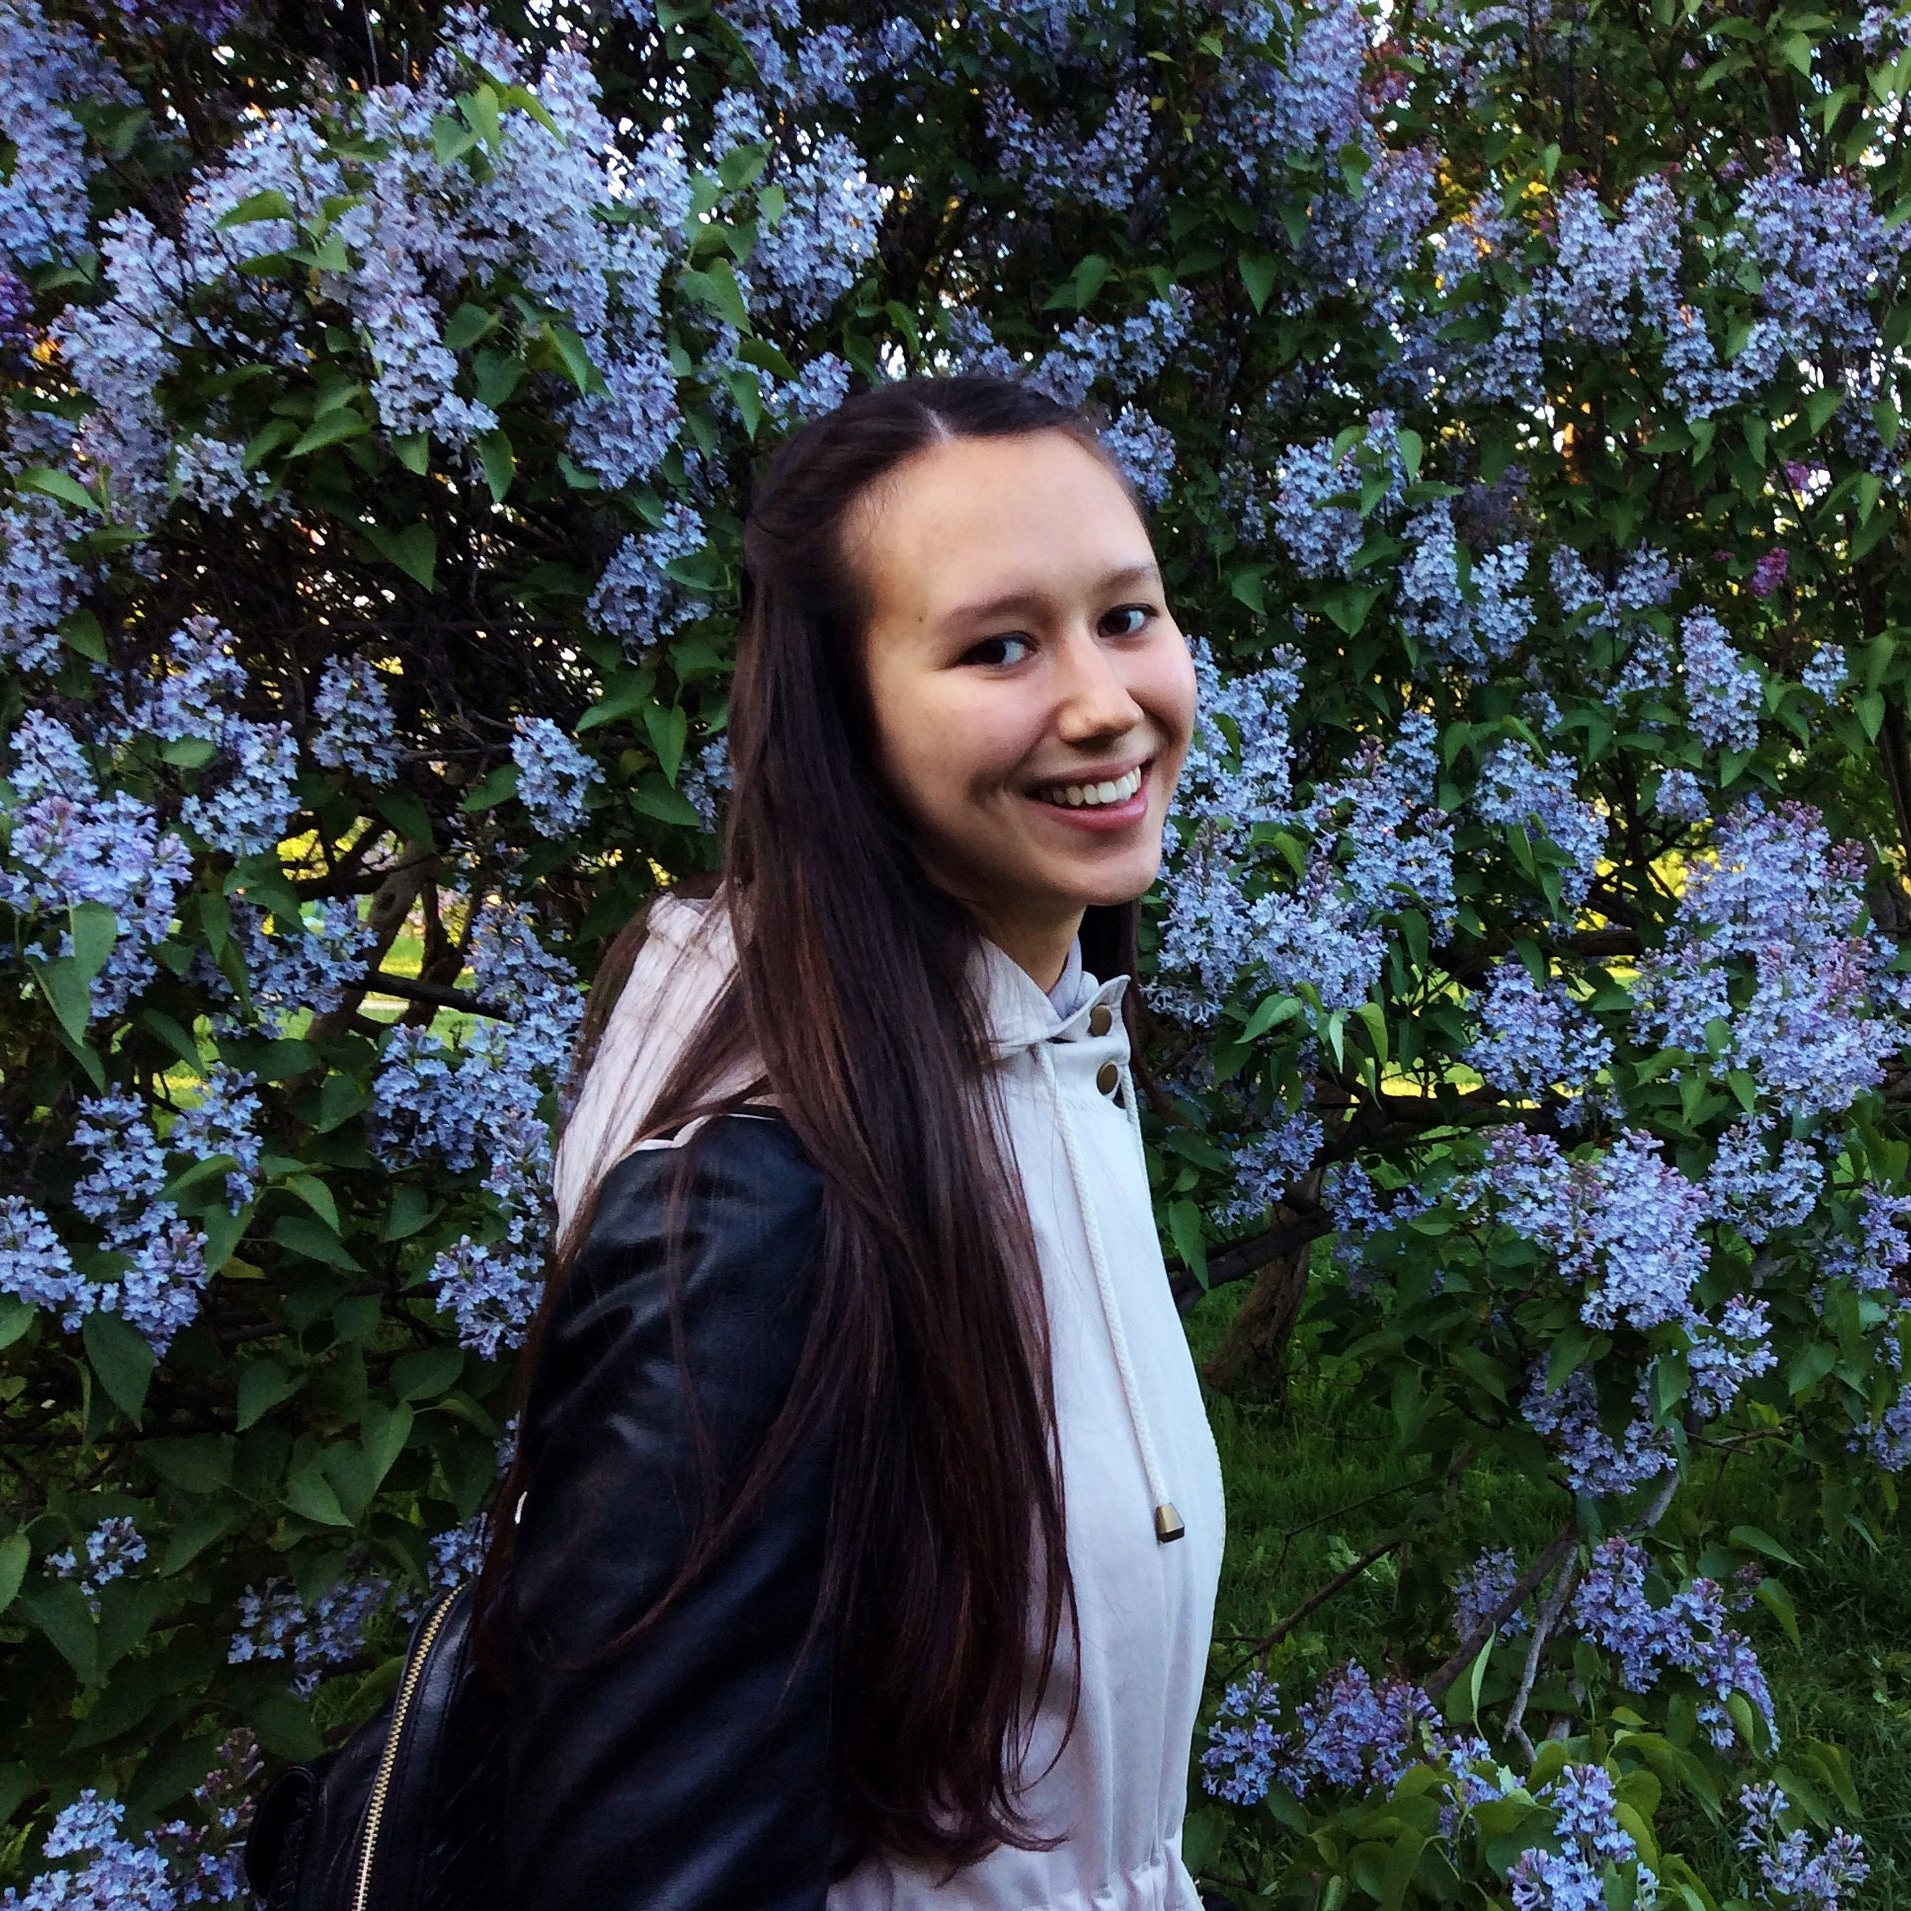
\includegraphics[scale=0.13]{Kam.jpg}


\section{Формулы}

\begin{equation}
S = \sqrt{p(p-a)(p-b)(p-c)}  \tag{\ae} \label{a}
\end{equation}

\begin{equation}
\frac{I_1}{I_2}=10^{ 0,4 \cdot (m_2-m_1) }\tag{\ae\ae}\label{aa}
\end{equation}

\begin{align*}
 & |A| = \begin{vmatrix}
  a_{1,1} & a_{1,2} & a_{1,3} \\
  a_{2,1} & a_{2,2} & a_{2,3} \\
  a_{3,1} & a_{3,2} & a_{3,3}
 \end{vmatrix} = \\
 & = a_{1,1} \cdot a_{2,2} \cdot a_{3,3} + a_{1,2} \cdot a_{2,3} \cdot a_{3,1} +a_{2,1} \cdot a_{3,2} \cdot a_{1,3} - \\
 & - a_{1,3} \cdot a_{2,2} \cdot a_{3,1} - a_{2,1} \cdot a_{1,2} \cdot a_{3,3} - a_{1,1} \cdot a_{3,2} \cdot a_{2,3}
 \tag{\ae\ae\ae} \label{a3}
\end{align*}

\begin{equation}
(a+b)^ n = \sum_{k=0}^{n} C_n^k a^k b^{n-k} \tag{\ae\ae\ae\ae} \label{a4}
\end{equation}

\begin{equation}
\int_{-\infty}^{+\infty} e^{-\frac{x^2}{2}} dx = \sqrt{2\pi} \tag{\ae\ae\ae\ae\ae} \label{a5}
\end{equation}

\begin{equation}
\displaystyle \lim_{n \to \infty} \frac{n!}{\sqrt{2 \pi n} \left(\frac{n}{e}\right)^n} = 1  \tag{\ae\ae\ae\ae\ae\ae} \label{a6}
\end{equation}

Каждая формула вызывает у меня воспоминания об определенных периодах моей жизни. Формула Геррона \eqref{a} является олицетворением школьной геометрии. Вторая формула Погсона \eqref{aa} напоминает мне о моей любви-астрономии, которой я занималась в конце школы. Следующие две формулы \eqref{a3} и \eqref{a4} из линейной алгебры и дискретной математики. Вспомнила первый курс, прослезилась. Последняя из любимых формул \eqref{a5} - следствие из интеграла Эйлера-Пуассона, который выручал на парах теории вероятности второго курса. Напротив, формула \eqref{a6} не оставляет положительных воспоминаний, да и тяжело мне запомнить этого Стирлинга.

\end{document} % конец документа